\documentclass{jarticle}
\usepackage{robomech}
\usepackage[dvipdfmx]{graphicx}
\usepackage{amsfonts}
\usepackage{hyperref}

\begin{document}
\makeatletter
\title{価値反復を用いた移動ロボットによる屋外ナビゲーション}
{}
{Outdoor navigation with a mobile robot using value iteration}
{}

\author{
	\begin{tabular}{ll}
		○学\hspace{1zw}登内 リオン(千葉工大)& 正\hspace{1zw}林原 靖男\hspace{1zw} (千葉工大)\\
 		\hspace{1zw}正\hspace{1zw}上田 隆一(千葉工大)\\
		% ※協賛・後援団体の会員資格で発表される場合は「正・学」は不要です。
	\end{tabular}
	% &\\
	\vspace{1zh} \\
	\begin{tabular}{l}
			{\small Leon TONOUCHI, Chiba Institute of Technology, s20c1078un@s.chibakoudai.jp} \\
			{\small Ryuichi UEDA, Chiba Institute of Technology} \\
			{\small Yasuo HAYASHIBARA, Chiba Institute of Technology}             \\
	\end{tabular}
}
\makeatother

\abstract{ \small
We examine our software package for mobile robot navigation in the real world. 
This software uses value iteration for updating a decision making policy 
in the whole state space. Though the computational cost of this method
is too large for current computers, we expect that it will be standard
in future. In the experiments, we use this package with a laptop computer on
a mobile robot. Though the calculation time is still a problem,  
it works on the mobile robot for the first time. 
}

\date{} % 日付を出力しない
\keywords{Autonomous mobile robots, Navigation, route planning generation}

\maketitle
\thispagestyle{empty}
\pagestyle{empty}

\small
\section{緒言}%===========================
%本文:明朝体・9pt(欧文Times New Roman, 9pt)、文字間隔は1行26文字程度、行間隔は4.2mm程度にして下さい。
価値反復は、最適制御理論を用いて、有限マルコフ決定過程における最適方策を正確に求めることができる手法である[1].
自律移動ロボットが実環境で走行することを考えると,変化する目的地や経路に対して即座に行動計画を必要となる.
例えば,運搬用の自律移動ロボットを考えると,目的地の到達したから即座に次の目的地への行動の計画が必要である.
さらに,安定した行動を計画しなければ,現場にいる同様のロボットや動く人に対応することが難しい.

価値反復を移動ロボットの行動計画に適用するとロボットの様々な状態に対して最適な行動を計算することができる[2].
しかし,実際のコスト(距離や時間)と事前情報から予測されるコストからひとつの経路を求めることを主な目的とした A*[3]よりも計算量が大きくなってしまう.

一方,上田らは価値反復を用いたナビゲーションは限られた環境の広さであれば利用できるのではないかと考え ROS パッケージを実装した[4].
このパッケージを用いると,ロボットが走行中,常に価値反復を行うため,計算量が多いが
\begin{itemize}
	\item 決められた行動の中で最適な経路を導出
	\item ロボットの様々な状態(位置や向き)での最適な行動を選択
 \end{itemize}
することができるでの,環境のあらゆる地点で最適な行動を計算可能である.そして100$\mathrm{[m^2]}$の広さのシミュレータ環境で2秒の計算コストで行動計画が可能であることが確認されている.

そこで本稿では,価値反復を用いた実時間経路計画アルゴリズムを屋外移動ロボットで用い,屋外の実環境を走行させ計算量を評価する.
このアルゴリズムを用いると理論上,最適な経路を得ることができるが計算量が大きいため,実機に適用できるか調査する.
%\subsection{論文作成に関する注意事項を以下に示します。(中見出し:ゴシック体・9pt・強調文字・左寄せ)}%-----------


%※ ただし、PDFファイルの容量は2MB以下、論文のページ数は2頁以上4頁以下とします。なお、印刷原稿の提出は不要ですので、郵送しないで下さい。

%※ 講演番号、講演会名、ページ番号は記載しないようにして下さい。
\section{実験}%===========================
今回の実験では上田らが開発したROSパッケージ(\href{https://github.com/ryuichiueda/value_iteration}{https://github.com/ryuichiueda/value\_iteration})[4]を実装し実験を行った.
本研究では千葉工業大学津田沼キャンパス内でロボット(Raspberry Pi Cat)を走行させ計算量を測定する.
地図のスタート地点から設定したゴール地点まで10回走行させ,価値反復の計算量を計測した.

計算機には CPU として Intel Core i7-11800H(8コア16スレッド), DRAM として DDR4-3200 64GB を用いた.
自己位置推定には上田らが作成したROSのemclパッケージ(\href{https://github.com/ryuichiueda/emcl}{https://github.com/ryuichiueda/emcl})[5],価値反復の際のコストの計算には占有格子地図を用いた.

Table 1 には,地図の大きさ,格子の解像度,ロボットが移動できる地図のセルの数,面積を記載する.
Table 2 には,価値反復の離散状態数と行動の数を記載する.
離散状態数は,今回用いる地図のセルの数に,θ 軸上の区分数(今回の実験では60)をかけたものである.
Table 3 には,6種類の行動と各行動の前進の速度と角速度を記載する.
この値は使用するロボットに合わせ,適切だと考えられる値に調整したものである.

\begin{table}[hbtp]
  \caption{configurations of the map}
  \centering
  \begin{tabular}{l|r}
    \hline
    map size & 294.3$\mathrm{[m]}$ × 199.95$\mathrm{[m]}$\\
    cell resolution &  0.15$\mathrm{[m]}$ × 0.15$\mathrm{[m]}$ \\
		number of cells & 2,615,346\\
    number of free cells & 165,076\\
		the area of the free cells & 3714.98$\mathrm{[m^2]}$\\
    \hline
  \end{tabular}
\end{table}

\begin{table}[hbtp]
	\caption{parameters for value iterations}
  \centering
  \begin{tabular}{l|r}
    \hline
    number of states & 156,920,760\\
    number of free states &  9,904,560\\
		number of actions & 6\\
    \hline
  \end{tabular}
\end{table}

\begin{table}[hbtp]
	\caption{type of actions}
	\centering
	\begin{tabular}{l|cc}
 		\hline
		& forward & angular \\
 		type & versity[m/s] & versity[deg/s] \\
 		\hline \hline
 		forward & 0.3 & 0.0 \\
 		backward & -0.2 & 0.0 \\
 		right & 0.0 & -20.0 \\
 		left & 0.0 & 20.0 \\
 		right forward & 0.2 & -20.0 \\
 		left forward & 0.2 & 20.0 \\
	 \hline
	\end{tabular}
\end{table}

\begin{figure}[h!]
  \centering
   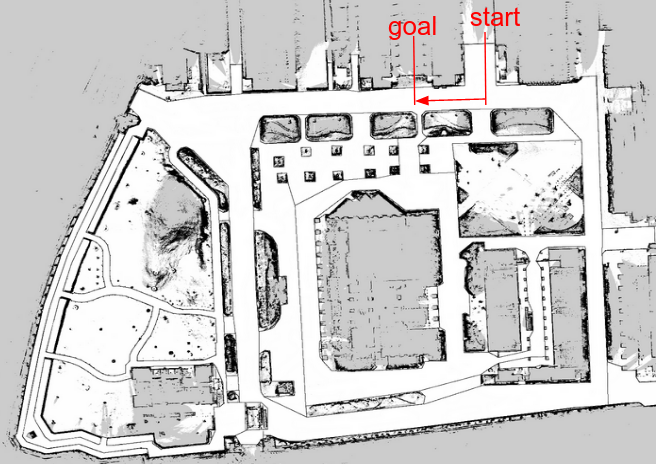
\includegraphics[height=40mm]{./figs/tsudanuma.png}
   \caption{the map for value iteration}
\end{figure}

\subsection{価値反復}
今回使用する価値反復のROSパッケージ[4]は,2次元の離散化した占有格子地図を読み込み,ロボットの向きの1次元を加えた3次元の離散空間で経路計画を行っている.
この離散空間を$\mathcal{S}$で表し,各区分$\mathit{s}\in\mathcal{S}$を離散状態と呼ぶ.
大域計画器は,次の2つの写像を出力する.
\begin{itemize}
	\item 最適状態価値関数$\mathit{V^*}$: $\mathcal{S}\rightarrow\mathbb{R}$
	\item 最適方策$\Pi\mathrm{^*}$: $\mathcal{S}\rightarrow\mathcal{A}$
\end{itemize}
$\mathcal{A}$は選択肢として用意された行動セット(Table3)のことである.
ある離散状態$\mathit{s}\in\mathcal{S}$の値$\mathit{V^*}(\mathit{s})$は,$\mathit{s}$から最適方策$\Pi\mathrm{^*}$に
したがって行動を取り続けた際のコストと移動時間の和の期待値である.
コストとは衝突の危険性などを時間の損失に換算し,数値化したものであり,占有格子地図から計算される,または人から与えられる.

\subsection{並列処理}
価値反復のノード(vi\_node)は,他のノードからゴールを指定されると即座に価値反復を開始する.
開始すると,自己位置推定のノードから出力されるロボットの推定姿勢のトピックを受けて,
その時点で得られる方策に基づいて行動(Table3)を選択し,選んだ行動に対応するロボットの速度を出力する.
価値反復のノードにはLinuxのPOSIXスレッドによる並列処理が導入されている.並列化されているのは,状態遷移確率を求める処理と価値反復を行う処理である.

状態遷移確率を求める処理は,ロボットが動作する前に一度だけ行うもので,スレッド数を多くしてCPUを使い切り短い時間で終わらせる実装になっている.
$\theta$軸の離散区間ごとにスレッドを用意する実装になっていて,今回の実験では区間の幅が6$\mathrm{[deg]}$で,区間数が60個なので60個のスレッドが同時に走る.

価値反復に用いるスレッドは設定で変更できるように実装されている.価値反復はロボットが動作しているときに実行されるため,
演算に使用するスレッド数を多くしてしまうと,センサ処理の遅延などの悪影響が生じてしまう.


\subsection{計算量の評価}
評価する方法としては,上田らの研究[4]と同様の方法を用いる.
しかし,スレッド数の増加によってナビゲーションにかかる時間が短縮すること,
そして,物理コア数以上のスレッド数を用いた場合,短縮の効果が頭打ちであるという結果がでているので,
本研究では使用する計算機の物理コア数が16コアであるため,スレッド数は16に固定して実験を行う.
\subsection{実験結果}
ロボットは価値反復の計算終了前に行動を開始するため,次のAとBの実験の時間の差から実質的な計算時間を評価する.
Table 4 に A と B のそれぞれの場合の実験結果を示す.
A と B の計測の内容は以下のとおりである.

\begin{itemize}
	\item A: 価値反復中からロボットを動作させて計測
	\item B: 価値反復が終了したあとにロボットを動作させて計測
\end{itemize}

\begin{table}[hbtp]
	\caption{computational complexity}
	\centering
	 \begin{tabular}{l|cc}
		\hline
		 & average & standard \\
		 & of total time[s] & deviation[s] \\
		\hline \hline
		A & 123.3 & 6.2 \\
		B & 207.8 & 2.2 \\
		\hline
	 \end{tabular}
 \end{table}

Table4には,Aの実験とBの実験それぞれでの計測した時間の平均と標準偏差を記載した.
Aの実験の平均時間とBの実験の平均時間の差より,今回の実験条件では実質的な価値反復の計算時間は84.6$\mathrm{[s]}$であった.

今回の実験では価値反復に用いる地図と自己位置推定に用いる地図の大きさを同じにしていた.
そのため自己位置推定に悪影響を及ぼさない大きさの地図を使って計算量の評価を行っていた.
しかし,現在の地図の大きさだと価値反復の計算に時間がかかり過ぎてしまう.
そのため,価値反復に用いる地図と自己位置推定に用いる地図を別々にすることで,価値反復に用いる地図を今以上に小さくすることができる.
地図を小さくすることで,離散状態数が減少し価値反復の計算にかかる時間が短くなると考えられる.
\section{結言}%===========================
本稿では,価値反復を用いた実時間経路計画アルゴリズムを屋外移動ロボットで用い,屋外の実環境を走行させることで計算量を評価した.
結果としては,3714.98$\mathrm{[m^2]}$のフリースペースがある環境において,地図の解像度を0.15$\mathrm{[m/pixel]}$,Intel Core i7-11800Hを有する計算機を用いると,
84.6$\mathrm{[s]}$も計算に時間がかかってしまうという結果が得られた.
結果から,屋外などの広い環境を想定した場合,今回の実験の条件では価値反復の計算に時間がかかり過ぎてしまうため,
屋外での走行を想定した移動ロボットへの適用は適切ではないと言える.

しかし,価値反復に使用する地図の解像度をできる限り下げることで,離散状態数が小さくなるので,価値反復の計算に用いる時間を短くすることができると考えられる.

今後は,価値反復に用いる地図の解像度をどこまで下げることで,屋外を想定した移動ロボットへの適用が可能になるのかということを調査する.

\footnotesize
\begin{thebibliography}{99}

	\bibitem{Shinjuku1}
	Bellman, R., ``{\it Dynamic Programming},'' Princeton Uni-versity Press, Princeton, NJ, 1957.

	\bibitem{Shinjuku2}
	上田隆一,池邉龍宏,林原靖男,``移動ロボットのナビゲーションのためのbrute-forceな価値反復を用いた大域計画・局所計画アルゴリズム'', 
	第27回ロボティクスシンポジア講演論文集, 2022.
	
	\bibitem{Shinjuku3}
	Hart, P. E., Nilsson, N. J. and Raphael, B. ``A Formal
	Basis for the Heuristic Determination of Minimal Cost
	Paths,'' {\it IEEE Transactions on Systems Science and Cybernetics}, Vol. 4, No. 2, pp. 100-107, 1968.
	
	\bibitem{Shinjuku4}
	上田隆一,池邉龍宏,林原靖男,``brute-forceな価値反復を用いた実時間経路計画ROSパッケージ'', 
	第39回日本ロボット学会学術講演会予稿集, 2021.

	\bibitem{Shinjuku5}
	Ueda, R., {\it et al}., ``Real-Time Decision Making with State-Value Function under Uncertainty of State Estimation,''
	 in {\it Proc. of} ICRA, 2005.

\end{thebibliography}

\normalsize
\end{document}
